% ======================= ХОД 1 =======================
\begin{figure}[H]
\centering
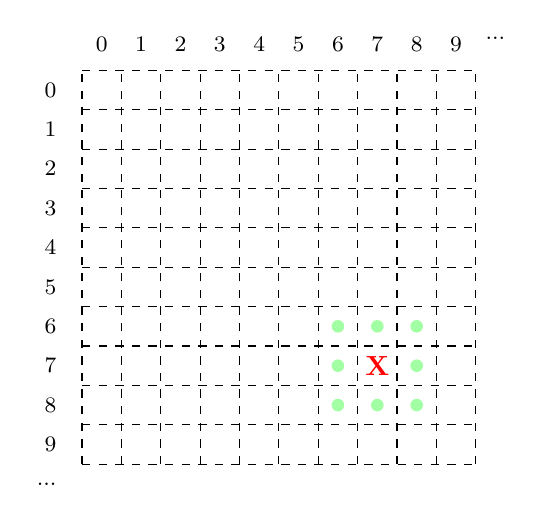
\begin{tikzpicture}[scale=0.5]
\draw[dashed,thin] (0,0) grid (10,10);
% Оси координат
\foreach \i in {0,...,9}
    \node[anchor=north] at (\i+0.5,11+.1) {\footnotesize\i};
\node[anchor=north] at (10+0.5,11+.1) {\footnotesize...};
\foreach \i in {0,...,9}
    \node[anchor=east] at (-0.4,9.5-\i) {\footnotesize\i};
\node[anchor=east] at (-0.4,9.5-10) {\footnotesize...};

% X
\node[scale=1,red] at (7.5,2.5) {\textbf{X}};
% Перспективные ходы вокруг X
\foreach \x/\y in {6.5/2.5,8.5/2.5,7.5/1.5,7.5/3.5,6.5/1.5,8.5/1.5,6.5/3.5,8.5/3.5}
    \fill[green!60!white,opacity=0.6] (\x,\y) circle (0.16);
\end{tikzpicture}
\caption{X ходит в центре (7,7), что обеспечивает максимальную свободу для дальнейших ходов.}
\end{figure}

% ======================= ХОД 3 =======================
\begin{figure}[H]
\centering
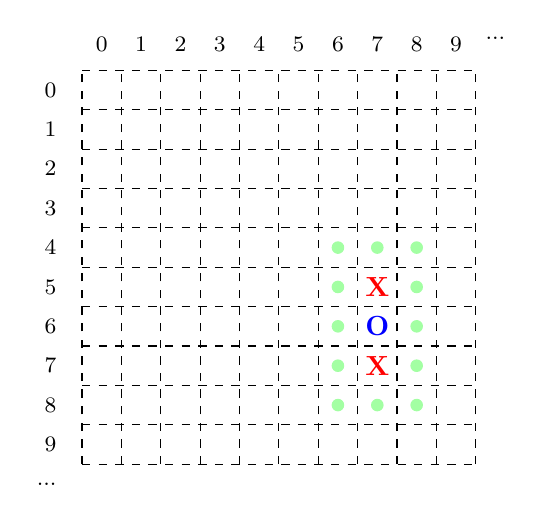
\begin{tikzpicture}[scale=0.5]
\draw[dashed,thin] (0,0) grid (10,10);
\foreach \i in {0,...,9}
    \node[anchor=north] at (\i+0.5,11+.1) {\footnotesize\i};
\node[anchor=north] at (10+0.5,11+.1) {\footnotesize...};
\foreach \i in {0,...,9}
    \node[anchor=east] at (-0.4,9.5-\i) {\footnotesize\i};
\node[anchor=east] at (-0.4,9.5-10) {\footnotesize...};

\node[scale=1,red] at (7.5,2.5) {\textbf{X}};
\node[scale=1,blue] at (7.5,3.5) {\textbf{O}};
\node[scale=1,red] at (7.5,4.5) {\textbf{X}};
% Перспективные: продолжаем строить вверх, наращиваем угрозу по вертикали
\foreach \x/\y in {7.5/1.5,6.5/2.5,8.5/2.5,6.5/1.5,8.5/1.5,6.5/3.5,8.5/3.5,6.5/4.5,8.5/4.5,7.5/5.5,6.5/5.5,8.5/5.5}
    \fill[green!60!white,opacity=0.6] (\x,\y) circle (0.16);
\end{tikzpicture}
\caption{X ходит в (7,5), O -- в (7,6).}
\end{figure}

% ======================= ХОД 5 =======================
\begin{figure}[H]
\centering
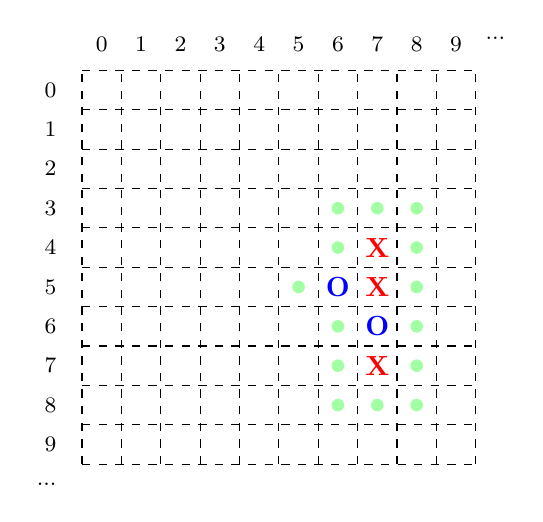
\begin{tikzpicture}[scale=0.5]
\draw[dashed,thin] (0,0) grid (10,10);
\foreach \i in {0,...,9}
    \node[anchor=north] at (\i+0.5,11+.1) {\footnotesize\i};
\node[anchor=north] at (10+0.5,11+.1) {\footnotesize...};
\foreach \i in {0,...,9}
    \node[anchor=east] at (-0.4,9.5-\i) {\footnotesize\i};
\node[anchor=east] at (-0.4,9.5-10) {\footnotesize...};

\node[scale=1,red] at (7.5,2.5) {\textbf{X}};
\node[scale=1,blue] at (7.5,3.5) {\textbf{O}};
\node[scale=1,red] at (7.5,4.5) {\textbf{X}};
\node[scale=1,blue] at (6.5,4.5) {\textbf{O}};
\node[scale=1,red] at (7.5,5.5) {\textbf{X}};
% Перспективные: можно завершать вертикаль, а также возможны ходы по диагоналям
\foreach \x/\y in {7.5/1.5,6.5/2.5,8.5/2.5,6.5/1.5,8.5/1.5,6.5/3.5,8.5/3.5,8.5/4.5,6.5/5.5,8.5/5.5,7.5/6.5,6.5/6.5,8.5/6.5,5.5/4.5}
    \fill[green!60!white,opacity=0.6] (\x,\y) circle (0.16);
\end{tikzpicture}
\caption{X ходит в (7,4), O -- в (6,5).}
\end{figure}

% ======================= ХОД 7 =======================
\begin{figure}[H]
\centering
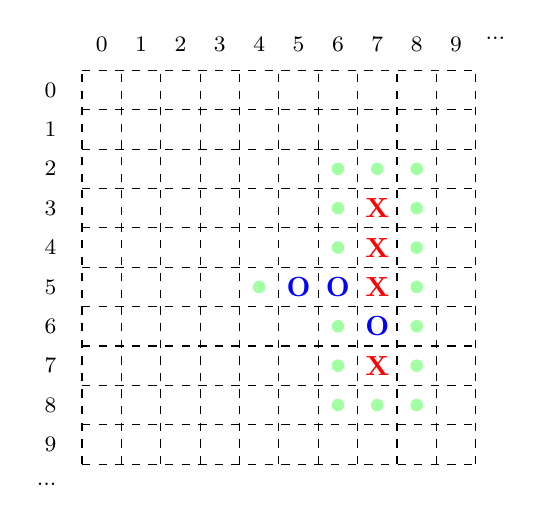
\begin{tikzpicture}[scale=0.5]
\draw[dashed,thin] (0,0) grid (10,10);
\foreach \i in {0,...,9}
    \node[anchor=north] at (\i+0.5,11+.1) {\footnotesize\i};
\node[anchor=north] at (10+0.5,11+.1) {\footnotesize...};
\foreach \i in {0,...,9}
    \node[anchor=east] at (-0.4,9.5-\i) {\footnotesize\i};
\node[anchor=east] at (-0.4,9.5-10) {\footnotesize...};

\node[scale=1,red] at (7.5,2.5) {\textbf{X}};
\node[scale=1,blue] at (7.5,3.5) {\textbf{O}};
\node[scale=1,red] at (7.5,4.5) {\textbf{X}};
\node[scale=1,blue] at (6.5,4.5) {\textbf{O}};
\node[scale=1,red] at (7.5,5.5) {\textbf{X}};
\node[scale=1,blue] at (5.5,4.5) {\textbf{O}};
\node[scale=1,red] at (7.5,6.5) {\textbf{X}};
% Перспективные: X почти выигрывает, остались ходы наверх или расширение по бокам
\foreach \x/\y in {7.5/1.5,6.5/2.5,8.5/2.5,6.5/1.5,8.5/1.5,6.5/3.5,8.5/3.5,8.5/4.5,6.5/5.5,8.5/5.5,7.5/7.5,6.5/7.5,8.5/7.5,6.5/6.5,8.5/6.5,4.5/4.5}
    \fill[green!60!white,opacity=0.6] (\x,\y) circle (0.16);
\end{tikzpicture}
\caption{X ходит в (7,3), O -- в (5,5).}
\end{figure}

% ======================= ХОД 9 =======================
\begin{figure}[H]
\centering
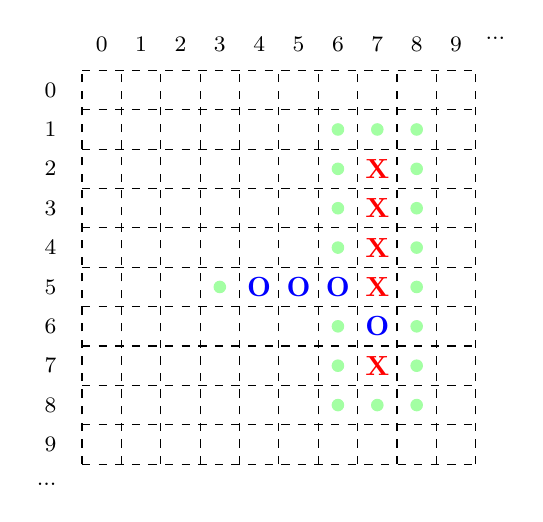
\begin{tikzpicture}[scale=0.5]
\draw[dashed,thin] (0,0) grid (10,10);
\foreach \i in {0,...,9}
    \node[anchor=north] at (\i+0.5,11+.1) {\footnotesize\i};
\node[anchor=north] at (10+0.5,11+.1) {\footnotesize...};
\foreach \i in {0,...,9}
    \node[anchor=east] at (-0.4,9.5-\i) {\footnotesize\i};
\node[anchor=east] at (-0.4,9.5-10) {\footnotesize...};

\node[scale=1,red] at (7.5,2.5) {\textbf{X}};
\node[scale=1,blue] at (7.5,3.5) {\textbf{O}};
\node[scale=1,red] at (7.5,4.5) {\textbf{X}};
\node[scale=1,blue] at (6.5,4.5) {\textbf{O}};
\node[scale=1,red] at (7.5,5.5) {\textbf{X}};
\node[scale=1,blue] at (5.5,4.5) {\textbf{O}};
\node[scale=1,red] at (7.5,6.5) {\textbf{X}};
\node[scale=1,blue] at (4.5,4.5) {\textbf{O}};
\node[scale=1,red] at (7.5,7.5) {\textbf{X}};
% Остальные перспективные — технические, игра завершилась бы победой X
\foreach \x/\y in {7.5/1.5,6.5/2.5,8.5/2.5,6.5/1.5,8.5/1.5,6.5/3.5,8.5/3.5,8.5/4.5,6.5/5.5,8.5/5.5,7.5/8.5,6.5/8.5,8.5/8.5,6.5/7.5,8.5/7.5,6.5/6.5,8.5/6.5,3.5/4.5}
    \fill[green!60!white,opacity=0.6] (\x,\y) circle (0.16);
\end{tikzpicture}
\caption{X ходит в (7,2), O -- в (4,5).}
\end{figure}

% ======================= ХОД 9 =======================
\begin{figure}[H]
\centering
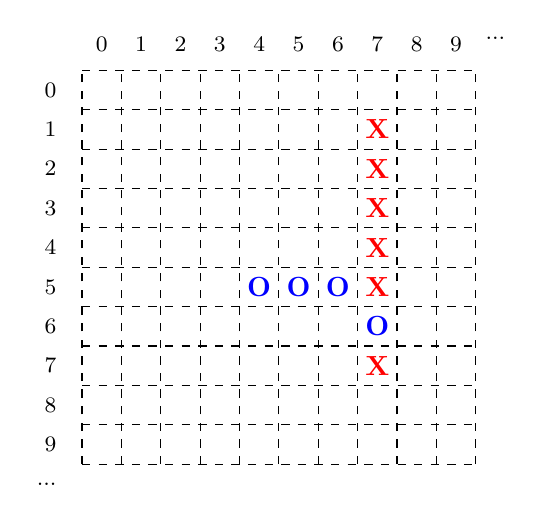
\begin{tikzpicture}[scale=0.5]
\draw[dashed,thin] (0,0) grid (10,10);
\foreach \i in {0,...,9}
    \node[anchor=north] at (\i+0.5,11+.1) {\footnotesize\i};
\node[anchor=north] at (10+0.5,11+.1) {\footnotesize...};
\foreach \i in {0,...,9}
    \node[anchor=east] at (-0.4,9.5-\i) {\footnotesize\i};
\node[anchor=east] at (-0.4,9.5-10) {\footnotesize...};

\node[scale=1,red] at (7.5,2.5) {\textbf{X}};
\node[scale=1,blue] at (7.5,3.5) {\textbf{O}};
\node[scale=1,red] at (7.5,4.5) {\textbf{X}};
\node[scale=1,blue] at (6.5,4.5) {\textbf{O}};
\node[scale=1,red] at (7.5,5.5) {\textbf{X}};
\node[scale=1,blue] at (5.5,4.5) {\textbf{O}};
\node[scale=1,red] at (7.5,6.5) {\textbf{X}};
\node[scale=1,blue] at (4.5,4.5) {\textbf{O}};
\node[scale=1,red] at (7.5,7.5) {\textbf{X}};
\node[scale=1,red] at (7.5,8.5) {\textbf{X}};
\end{tikzpicture}
\caption{X выигрывает -- ходит в (7,1).}
\end{figure}

